\section{PCL}

% \begin{frame}
%     \frametitle{Overview of Prosody Consistency Learning (PCL)}
%     The Prosody Consistency Learning (PCL) module aims to enhance the audiovisual consistency of dubbing.
%     \begin{itemize}
%         \item \textbf{Method:} Model phoneme-level prosody attributes using emotional facial expression information. It is mainly divided into the following two parts:
%         \begin{columns}[T] % Use top-aligned two columns
%             \column{0.55\textwidth} % Left column width is half of the text width
%             \begin{itemize}
%                 \item \textbf{Alignment of Emotion and Prosody Attributes:} Align the emotional state of the character with the phoneme-level prosody attributes of dubbing through emotion feature extraction and cross-modal attention mechanism.
%                 \item \textbf{Timbre Consistency:} Ensure that the generated dubbing maintains timbre consistency with the reference audio through timbre feature extraction and Timbre-Adaptive Layer Normalization (TALN).
%             \end{itemize}
%             \column{0.45\textwidth} % Right column width is half of the text width
%             \begin{figure}[htpb]
%                 \centering
%                 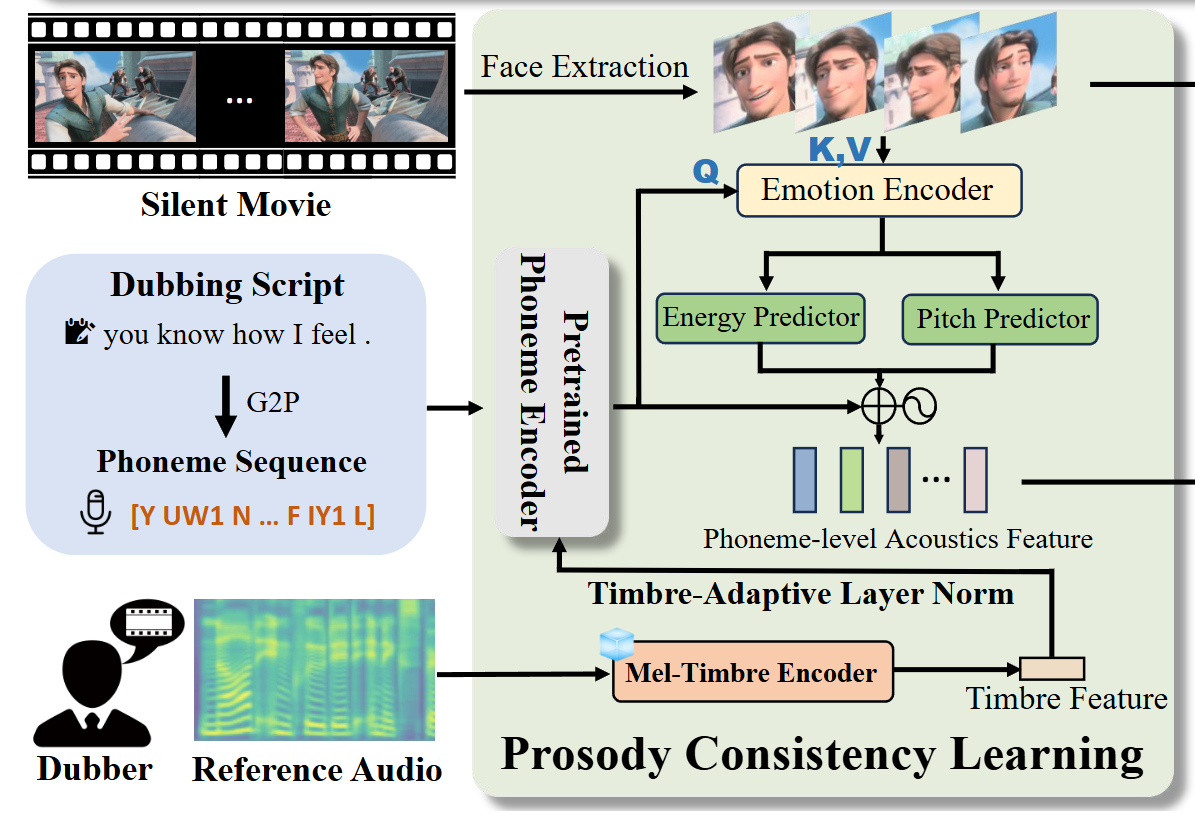
\includegraphics[width=\linewidth]{figs/PCL.png} % Replace with your image path
%                 \caption{Illustration of the PCL module}
%                 \label{fig:pcl-diagram}
%             \end{figure}
%         \end{columns}
%     \end{itemize}
% \end{frame}
\begin{frame}
    \frametitle{Overview of Prosody Consistency Learning (PCL)}
    \textbf{Objective:} Enhance audiovisual consistency of dubbing.
    \begin{itemize}
        \item \textbf{Method:} Model phoneme-level prosody using emotional facial expressions. Key components:
        \begin{columns}[c] % Use top-aligned two columns
            \column{0.55\textwidth} % Left column width
            \begin{itemize}
                \item \textbf{Emotion-Prosody Alignment:} Align character emotions with phoneme-level prosody via cross-modal attention.
                \item \textbf{Timbre Consistency:} Maintain reference audio's timbre using TALN.
            \end{itemize}
            \column{0.45\textwidth} % Right column width
            \begin{figure}
                \centering
                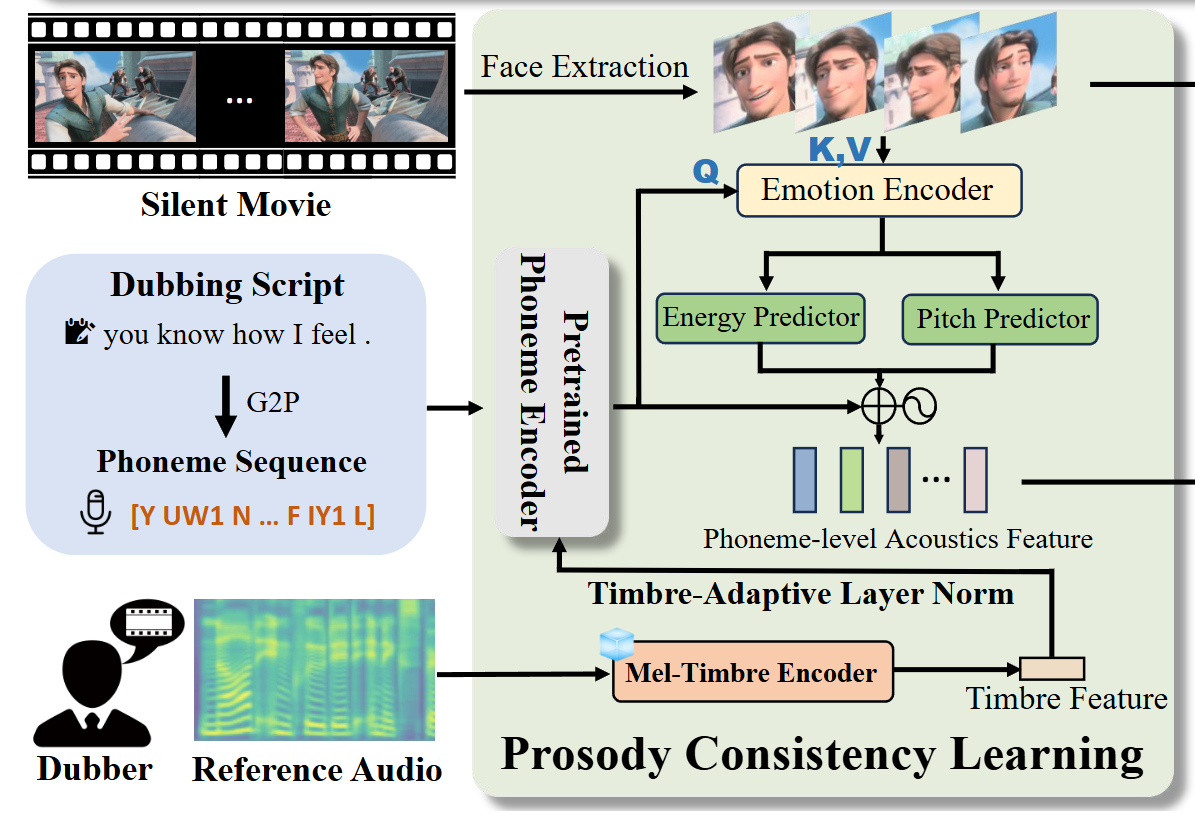
\includegraphics[width=\linewidth]{figs/PCL.png}
                \caption{PCL module illustration}
                \label{fig:pcl-diagram}
            \end{figure}
        \end{columns}
    \end{itemize}
\end{frame}


% \begin{frame}{Prosody Consistency Learning (PCL)}
% \framesubtitle{(1) Alignment of Emotion and Prosody Attributes}
% \begin{itemize}
%     \item \textbf{Objective:} Align the emotional state of the character in the movie clip with the phoneme-level prosody attributes (pitch and energy) of the dubbing while ensuring that the timbre of the dubbing remains consistent with the reference audio.
%     \item \textbf{Steps Introduction:}
%     \begin{enumerate}
%         \item \textbf{Emotion Feature Extraction:} Extract and encode emotional features from facial regions.
%         \item \textbf{Cross-modal Attention Mechanism:} Use attention mechanisms to align emotional features with phoneme prosody attributes.
%         \item \textbf{Prediction of Phoneme Pitch and Energy:} Predict the pitch and energy of phonemes and embed them into the phoneme sequence.
%     \end{enumerate}
%     \item \textbf{Step 1: Emotion Feature Extraction}
%     \begin{itemize}
%         \item Extract the facial region of each frame in the movie clip using S3FD face detection:
%         \begin{equation}
%             V_{\text{face}} = S^3FD(V_{\text{Ref}}) \in \mathbb{R}^{L_v \times H_{\text{face}} \times W_{\text{face}} \times C}
%         \end{equation}
%         \item Encode the facial region into emotional features using the EmoFAN network:
%         \begin{equation}
%             V_{\text{emo}} = \text{EmoFAN}(V_{\text{face}}) \in \mathbb{R}^{L_v \times d_m}
%         \end{equation}
%     \end{itemize}
% \end{itemize}
% \end{frame}
\begin{frame}{Prosody Consistency Learning (PCL)}
\framesubtitle{(1) Alignment of Emotion and Prosody Attributes}
\begin{itemize}
    \item \textbf{Objective:} Align character emotions with phoneme-level prosody (pitch and energy) while maintaining reference audio's timbre.
    \item \textbf{Steps:}
    \begin{enumerate}
        \item \textbf{Extract Emotion Features:} Detect faces with S3FD, encode emotions with EmoFAN.
        \item \textbf{Cross-modal Attention:} Align emotion features with phoneme prosody.
        \item \textbf{Predict Phoneme Attributes:} Embed predicted pitch and energy into phoneme sequence.
    \end{enumerate}
    \item \textbf{Step 1: Emotion Feature Extraction}
    \begin{itemize}
        \item Detect facial regions using S3FD:
        \begin{equation}
            V_{\text{face}} = S^3FD(V_{\text{Ref}}) \in \mathbb{R}^{L_v \times H_{\text{face}} \times W_{\text{face}} \times C}
        \end{equation}
        \item Encode emotions using EmoFAN:
        \begin{equation}
            V_{\text{emo}} = \text{EmoFAN}(V_{\text{face}}) \in \mathbb{R}^{L_v \times d_m}
        \end{equation}
    \end{itemize}
\end{itemize}
\end{frame}

\begin{frame}{Prosody Consistency Learning (PCL)}
\framesubtitle{(1) Alignment of Emotion and Prosody Attributes}

\begin{itemize}
    \item \textbf{Step 2: Cross-modal Attention Mechanism}
    \begin{itemize}
    \item Use multi-head cross-modal attention to align the emotional features of the character with the prosody attributes of each phoneme:
        \begin{equation}
            \xi_{\text{pho,pitch}}^k = \text{softmax}\left(\frac{Q^{\top} K_p}{\sqrt{d_m}}\right) V_p \in \mathbb{R}^{L_p \times \frac{d_m}{n_{\text{head}}}}
        \end{equation}
        \begin{equation}
            \xi_{\text{pho,energy}}^k = \text{softmax}\left(\frac{Q^{\top} K_e}{\sqrt{d_m}}\right) V_e \in \mathbb{R}^{L_p \times \frac{d_m}{n_{\text{head}}}}
        \end{equation}
        \item Where:
        \begin{equation}
            Q = W_j^Q T_e^{\top}, \quad K_p = W_j^{K_p} V_{\text{emo}}^{\top}, \quad V_p = W_j^{V_p} V_{\text{emo}}^{\top}
        \end{equation}
        \begin{equation}
            K_e = W_j^{K_e} V_e^{\top}, \quad V_e = W_j^{V_e} V_{\text{emo}}^{\top}
        \end{equation}
    \end{itemize}
\end{itemize}
\end{frame}


\begin{frame}{Prosody Consistency Learning (PCL)}
\framesubtitle{(1) Alignment of Emotion and Prosody Attributes}

\begin{itemize}
    \item  \textbf{Step 3: Prediction of Phoneme Pitch and Energy}
    \begin{itemize}
        \item Use pitch and energy predictors to predict the pitch and energy of each phoneme, convert them into pitch and energy embeddings, and then add them to the phoneme sequence:
        \begin{equation}
            \tilde{P}_{\text{pho}}, \tilde{E}_{\text{pho}} = \text{Predictor}(\xi_{\text{pho,pitch}}, \xi_{\text{pho,energy}}) \in \mathbb{N}^{L_p}
        \end{equation}
        \item Add pitch and energy embeddings to the phoneme sequence:
        \begin{equation}
            T_a = T_e + \text{PitchEmb}(\tilde{P}_{\text{pho}}) + \text{EnergyEmb}(\tilde{E}_{\text{pho}})
        \end{equation}
    \end{itemize}
\end{itemize}
\end{frame}


% \begin{frame}{Prosody Consistency Learning (PCL)}
% \framesubtitle{(2) Timbre Consistency}
% \begin{itemize}
%     \item \textbf{Objective:} Accurately replicate the timbre of the reference audio.
%     \item \textbf{Method:} Use Timbre-Adaptive Layer Normalization (TALN) to integrate the timbre feature into phoneme encoding and mel-spectrogram generation by predicting the gain and bias of the input vector sequence.
%     \item \textbf{Formula:}
%     \begin{equation}
%         \text{TALN}(x, E_{\text{timbre}}) = \text{gain}(E_{\text{timbre}}) \frac{x - \mu}{\sigma} + \text{bias}(E_{\text{timbre}})
%     \end{equation}
%     \item \textbf{Parameter Explanation:}
%     \begin{itemize}
%         \item \( x \) and \( E_{\text{timbre}} \) are the input sequence and timbre feature, respectively.
%         \item \( \mu \), \( \sigma \) are the mean and variance of \( x \), respectively.
%         \item \( \text{gain}(\cdot) \) and \( \text{bias}(\cdot) \) are the prediction functions for gain and bias, respectively.
%     \end{itemize}
%     \item \textbf{Application:} The proposed TALN is applied to each FFT block of the phoneme encoder and mel-decoder to integrate the vocal timbre feature.
% \end{itemize}
% \end{frame}

\begin{frame}{Prosody Consistency Learning (PCL)}
\framesubtitle{(2) Timbre Consistency}
\begin{itemize}
    \item \textbf{Objective:} Replicate reference audio's timbre accurately.
    \item \textbf{Method:} Use TALN to integrate timbre features into phoneme encoding and mel-spectrogram generation.
    \item \textbf{Formula:}
    \begin{equation}
        \text{TALN}(x, E_{\text{timbre}}) = \text{gain}(E_{\text{timbre}}) \frac{x - \mu}{\sigma} + \text{bias}(E_{\text{timbre}})
    \end{equation}
    \item \textbf{Parameters:}
    \begin{itemize}
        \item \( x \): Input sequence.
        \item \( E_{\text{timbre}} \): Timbre feature.
        \item \( \mu \), \( \sigma \): Mean and variance of \( x \).
        \item \( \text{gain}(\cdot) \), \( \text{bias}(\cdot) \): Predicted gain and bias.
    \end{itemize}
    \item \textbf{Application:} Apply TALN to each FFT block of phoneme encoder and mel-decoder.
\end{itemize}
\end{frame}